\section{Background}
\label{sec:background}
Recluse aims to preserve the users' privacy by hiding the users' traces from both IdP and RPs in SSO systems (e.g., the widely adopted OIDC SSO systems), with the basic requirements of SSO systems under consideration. In this paper, we focus on the OIDC implicit flow to present the necessary background information  and the basic requirements of SSO systems.
%This section adopts OIDC as the example to present the necessary background information  and the security consideration of SSO sytems.


%Recluse is an extension of OIDC to prevent the IdP from inferring the user's accessed RP, with the security of SSO systems under consideration.
%provides the necessary background information about OIDC and  the security consideration of SSO systems.
%Most of current IdPs\cite{Facebook} for web application use OAuth 2.0 authorization code flow. Because authorization code flow requires RP's secret for token exchanging. It actually achieves the binding of RP and access token. Although OAuth 2.0 implicit flow is not secure in authentication, many IdPs also use its modified version designed by each IdP for authentication.
%In this section, we firstly describe how OpenID Connect is defined. Then the discussion of SSO system is to illustrate that why OpenID Connect is chosen and the challenges and solutions of protecting user's privacy.

\subsection{OpenID Connect}
\label{subsec:OIDC}
Typical SSO systems~\cite{SAMLIdentifier,OpenIDConnect,SPRESSO} contain the following entities:
%The OIDC or OAuth systems contains following entities:
\begin{itemize}
    \item \textbf{IdP}. IdP maintains the user's attributes and credentials, performs the user authentication, generates the identity proof, binds it with the RP and sends the poof  to the correct RP through the user. The generation of identity proof is processed differently in various SSO systems. For example, in OIDC, IdP generates a PPID for the user's first login at a RP, checks the consistency of the RP's information (the URL and identifier) between ones from the maintained database and the request, and requires the  consent from the user about the exposed attributes.
     \item \textbf{User}. This entity completes the authentication at the IdP with securely maintained credentials, initiates a SSO process by requiring to login at a RP, relays the identity proof request from the RP to IdP, checks the scope of attributes exposed to RP, and transmits the identity proof from IdP to the RP correctly. Usually, these processes are handled by  a user-controlled software (e.g., the browser), called user agent.
    \item \textbf{RP}. RP provides the individual services to user based on the identifier from the identity proof. In details, RP constructs the identity proof request, sends the request to the IdP through the user, checks the correctness of the received identity proof, and parses the proof for necessary information. The details process varies in different systems. For example, in OIDC, RP needs to register at the IdP for the identifier to be used in the construction of the identity proof request, and derives the user's account based on PPID.
\end{itemize}
\begin{comment}
\begin{itemize}
    \item \textbf{User}. is the entity to be authenticated in this system who holds the credentials for the IdP. User takes part in the the system through the user agent. User agent is the software used by the user, such as browser and the application on the mobile device, which is required to transmit the authentication request and identity proof between IdP and RP correctly.
     \item \textbf{IdP}. is the entity who authenticates the user and provide the identity proof. IdP authenticates the user, verifies the authentication request from RP, generates user's PPID and issues the identity proof signed with its private key. Besides, IdP provides the notification to user about the range of exposed attributes to RP and guarantees that the identity proof should only be sent to the corresponding RP.
    \item \textbf{RP}. is the entity who provides the service and need to identify the user. RP builds the authentication request to IdP with its identifier and endpoint for identity proof. RP identifies a user through the PPID in identity proof.
\end{itemize}
\end{comment}


OpenID Connect (current version 1.0), a typical SSO standard,  defines the process at each entity and the protocol flows between entities. OIDC is  an extension of OAuth (current version 2.0). OAuth is originally designed for authorizing the RP to obtain the user's personal protected resources stored at the resource holder. That is, the RP obtains an access token generated by the IdP after a clear consent from the user, and  uses the access token to obtain the specified resources of the user from the resource holder. However, plenty of RPs adopt OAuth 2.0 in the user authentication, which is not formally defined in the specifications~\cite{rfc6749,rfc6750}, and makes impersonation attack possible~\cite{ChenPCTKT14, WangZLG16}. For example, the access token isn't required to be bound with the RP, the adversary may act as an RP to obtain the access token and use it to impersonate as the victim user in another RP.

%OpenID Connect (current version 1.0) is an extension of OAuth (current version 2.0). OAuth is originally designed for authorizing the RP to obtain the user's personal protected resources stored at the resource holder. That is, the RP obtains an access token generated by the resource holder after a clear consent from the user, and  uses the access token to obtain the specified resources of the user from the resource holder. However, plenty of RPs adopt OAuth 2.0 in the user authentication, which is not formally defined in the specifications~\cite{rfc6749,rfc6750}, and makes impersonation attack possible~\cite{ChenPCTKT14, WangZLG16}. For example, the access token isn't required tp be bound with the RP, the adversary may act as a RP to obtain the access token and use it to impersonate as the victim user in another RP.


%OAuth 2.0 is specifically designed for user authorization. It allows third party to access user's personal protected resources from resource holder. In OAuth 2.0 system everyone carrying user's access token is able to achieve user's protected resources from resource holder. Access token is not bound with any RP so that it is not appropriate for authentication. OpenID Connect offers an additional id token for user identifying so that it can be used in both authentication and authorization.

%OpenID Connect 1.0 is an extension of OAuth 2.0. OAuth 2.0 is specifically designed for user authorization. It allows third party to access user's personal protected resources from resource holder. In OAuth 2.0 system everyone carrying user's access token is able to achieve user's protected resources from resource holder. Access token is not bound with any RP so that it is not appropriate for authentication. OpenID Connect offers an additional id token for user identifying so that it can be used in both authentication and authorization.

OIDC is designed to extend OAuth for user authentication,
% by binding the identity proof for authentication with the information of RP.
 which provides three protocol flows: authorization code flow, implicit flow and hybrid flow (i.e., a mix-up of the previous two flows). In the authorization code flow, the identity proof is the authorization code sent by the IdP, which is bound with the RP, as only the target RP is able to obtain the user's attributes with this authorization code and the corresponding secret (distributed in the RP's registration) which is performed in the similar way as the authentication in OAuth 2.0.

The implicit flow of OIDC achieves the binding between the identity proof and the RP, by using the new id token as the identity proof. In details, id token includes the user's PPID, the RP's identifier (RPID), the issuer, issuing time, the validity period and the other requested attributes. The IdP completes the construction of the id token by generating the signature of these elements with its private key, and sends it to the RP previously registered endpoint. The RP validates the id token, by verifying the signature with the IdP's public key, checking the correctness of the valid period and the consistency of RPID with the identifier stored locally. Figure~\ref{fig:OpenID} provides the details in the implicit flow of OIDC. The detailed processes are as follows:
\begin{itemize}
    \item Step 1: User attempts to login at one RP.
    \item Step 2: The RP redirects the user to the corresponding IdP with a newly constructed request of identity proof. The request contains RPID, the registered endpoint, and the set of requested attributes.
    \item Step 3: If the user hasn't been authenticated, an extra authentication process is performed.
    \item Step 4, 5: The IdP generates the identity proof for the user who has been authenticated already and constructs the response with endpoint in request if it is the same with the registered one for the RP.
    \item Step 6, 7: The RP verifies the id token, identifies the user with PPID in the id token, and returns the authentication result to user.
\end{itemize}

\begin{comment}
The implicit flow of OIDC achieves the binding between the identity proof and the RP, by introducing a new token (i.e., id token). In details, id token includes the user's PPID (i.e., \verb+sub+), the RP's identifier (i.e., \verb+aud+), the issuer, issuing time, the validity period and the other requested attributes. The IdP completes the construction of the id token by generating the signature of these elements with its private key, and sends it to the correct RP through the redirect URL registered previously.  The RP validates the id token, by verifying the signature with the IdP's public key, checking the correctness of the valid period and the consistency of \verb+aud+ with the identifier stored locally. Figure~\ref{fig:OpenID} provides the details in the implicit flow of OIDC, where the dashed lines represent the message transmission  in  the browser while the solid lines denote the network traffic. The detailed processes are as follows:
\begin{itemize}
    \item Step 1: User attempts to login at one RP.
    \item Step 2: The RP redirects the user to the corresponding IdP with a newly constructed request of id token. The request contains RP's identifier (i.e., \verb+client_id+), the endpoint (i.e., \verb+redirect_uri+) to receive the id token, and the set of requested attributes (i.e., \verb+scope+). Here, the \verb+openid+ should be included in \verb+scope+ to request the id token.
    \item Step 3: The IdP generates the id token and the access token for the user who has been authenticated already, and constructs the response with  endpoint (i.e., \verb+redirect_uri+)  in request if it is the same with the registered one for the RP. If the user hasn't been authenticated, an extra authentication process is performed.
    \item Step 4, 5: The RP verifies the id token, identifies the user with \verb+sub+ in the id token, and requests the other attributes from IdP with the access token.
\end{itemize}
\end{comment}
\begin{figure}
  \centering
  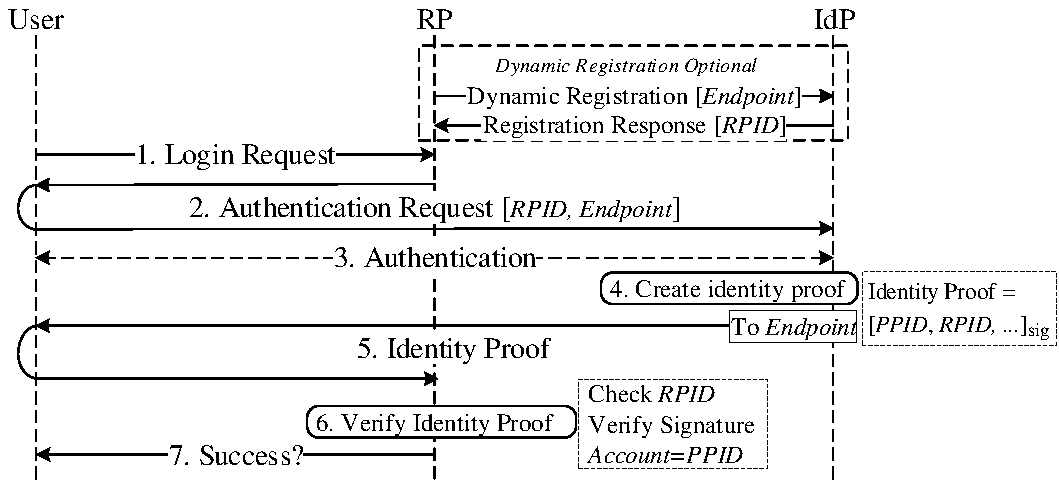
\includegraphics[width=\linewidth]{fig/OIDC1.pdf}
  %\subfigure[Authorization Code Flow]{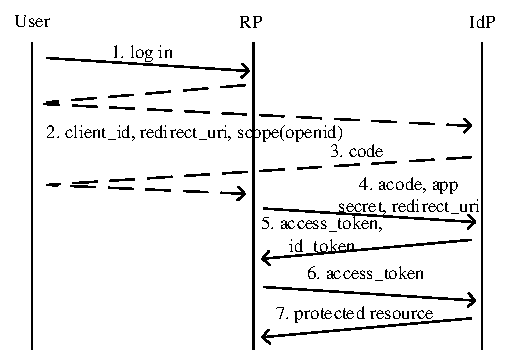
\includegraphics[width=\linewidth]{fig/openidconnect2.pdf}\label{fig:OpenID_code}}
  %\subfigure[Hybrid Flow]{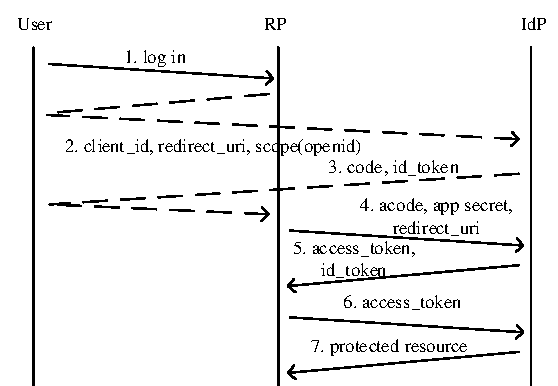
\includegraphics[width=\linewidth]{fig/openidconnect3.pdf}\label{fig:OpenID_hybrid}}
  \caption{The implicit protocol flow of OIDC.}
  \label{fig:OpenID}
\end{figure}

\begin{figure}
  \centering
  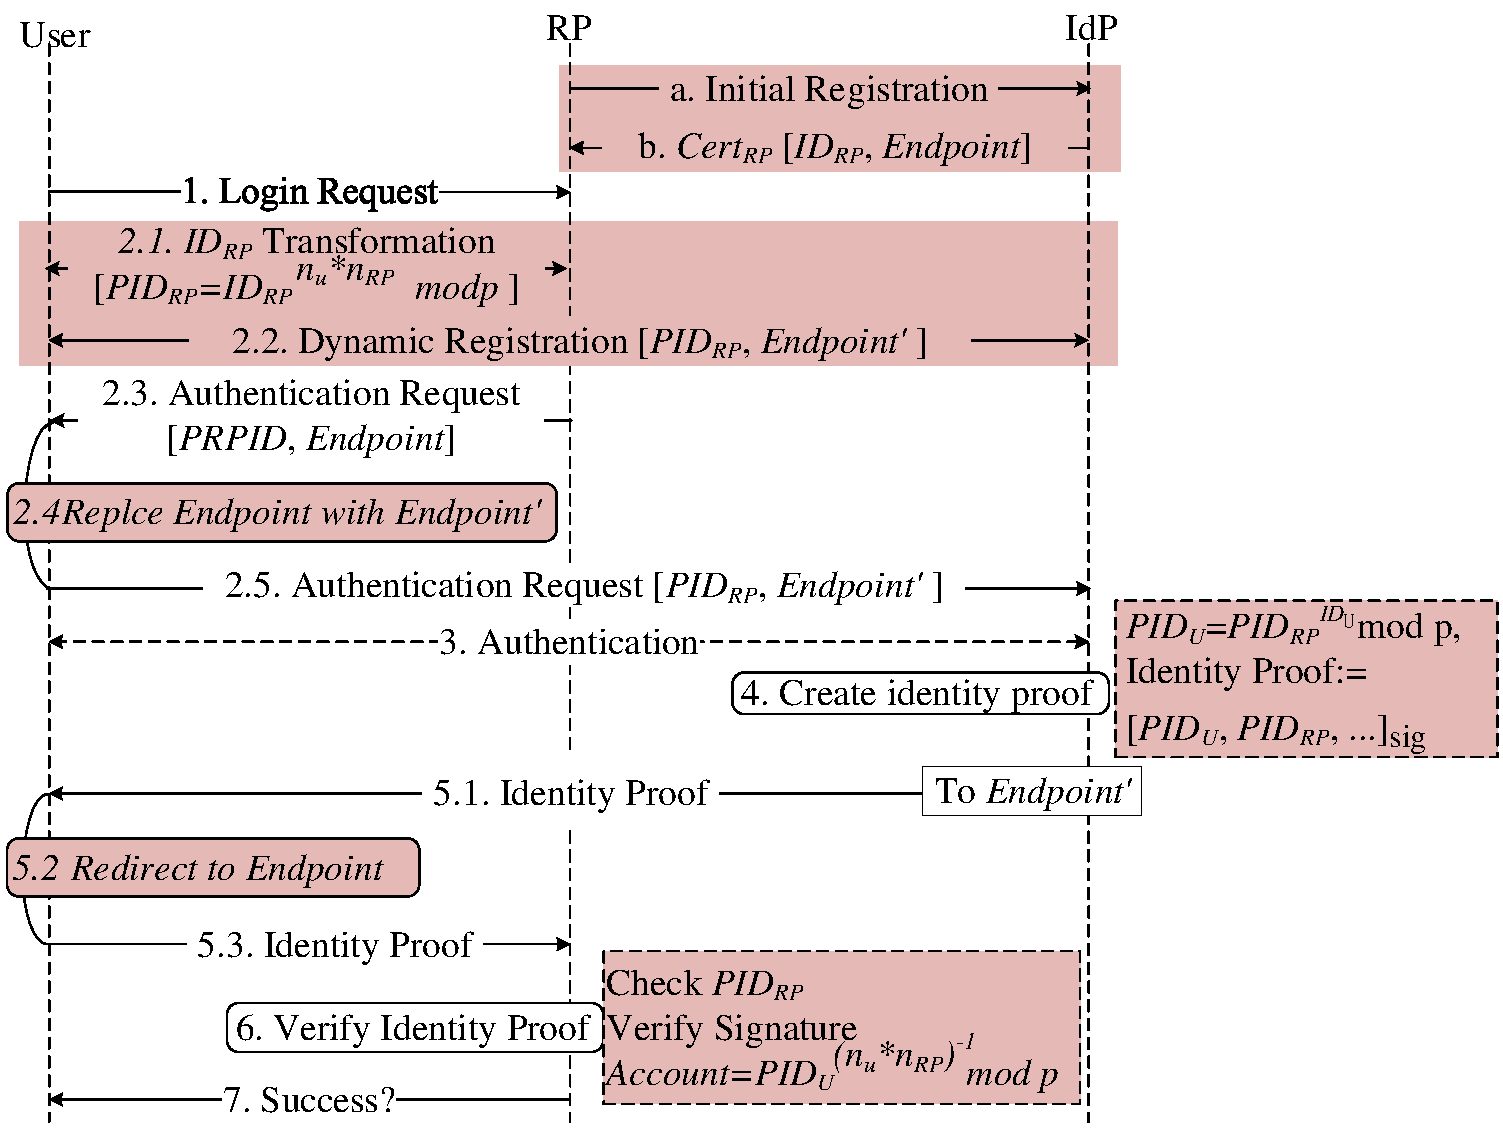
\includegraphics[width=\linewidth]{fig/overview1.pdf}
  %\subfigure[Authorization Code Flow]{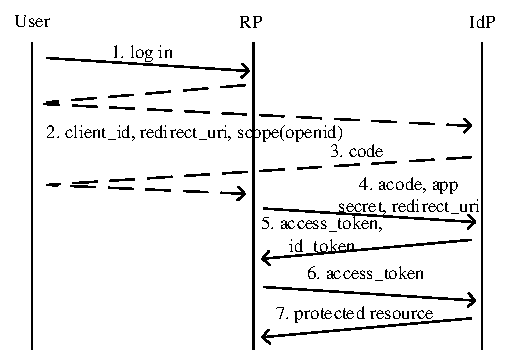
\includegraphics[width=\linewidth]{fig/openidconnect2.pdf}\label{fig:OpenID_code}}
  %\subfigure[Hybrid Flow]{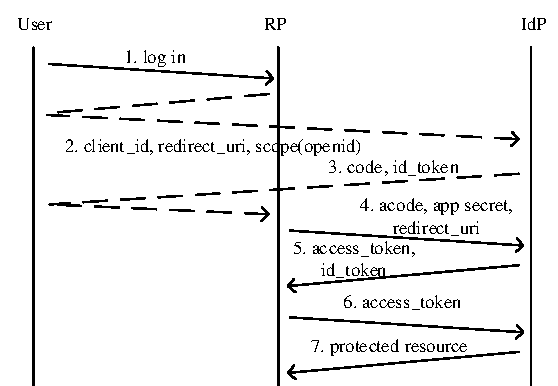
\includegraphics[width=\linewidth]{fig/openidconnect3.pdf}\label{fig:OpenID_hybrid}}
  \caption{The Recluse.}
  \label{fig:Recluse}
\end{figure}

\noindent\textbf{Dynamic Registration.} OIDC provides the dynamic registration~\cite{DynamicRegistration} mechanism to register the RP for a new RPID dynamically, shown in Figure~\ref{fig:OpenID}. After the first successful registration, RP obtains a registration token from the IdP, and is able to update its information (e.g., the endpoint) by a dynamic registration process with the  registration token. One successful dynamic registration process will make the IdP assign a new unique RPID for this RP.


\subsection{Basic Requirements of SSO}
\label{subsec:basicrequirements}
Based on the desiring function and the security analysis of SSO systems, we conclude the basic requirements of SSO. As our work is focused on the implicit flow of OIDC, the following requirements are illustrated based on the implicit flow of OIDC.
The requirements are shown as follows:
\begin{itemize}
\item[1.] \textbf{Identification}. Identification is the main feature of SSO system, which enables the RP to identify the user. Moreover, for web application, it is necessary to provide continuous and personalize service, which requires the RP to link the user with the specific account in RP. Therefore, the identity proof provided by the IdP must be linkable in the destination RP. That is, some of the existing SSO systems provide the pairwise identifier (e.g., PPID in OIDC) and others provide the unchanged identifier (e.g., email in SPRESSO) within the identity proof, all of which are unchanged for one user in one RP.
\item[2.] \textbf{Binding}. The identity proof should be bound with only one RP and accepted only by this RP, no other honest RP may accept this identity proof. Otherwise, the adversary may impersonate as the victim user, for example, by pretending as a RP to collect the victim's identity proof and using it at any other honest RP~\cite{ChenPCTKT14, WangZLG16}.
        Currently, the binding is achieved based on the claim in the identity proof, IdP claims the destination RP's identifier in the identity proof and avoids the modification on it by generating a signature, while the RP checks the RP's identifier and only accepts the identity proof for it.
\item[3.] \textbf{Confidentiality}. The identity proof should only be obtained by the correct RP (and the user), no one else may get the identity proof~\cite{ChenPCTKT14,FettKS16,WangZLG16}. Otherwise, the adversary may use the obtained identity proof to login as the victim user on the specified RP. To avoid the unauthorized leakage of identity proof, (1) the  user and IdP should perform additional checks  in its generation and transmit to ensure that the identity proof is generated for the correct RP (i.e., the correct identifier) and sent to the exact RP (i.e., correct URL); (2) TLS is adopted to ensure the confidentiality during transmit; (3) a trusted user agent is deployed to ensure the identity proof is only sent to the URL specified by the IdP.
\item[4.] \textbf{Integrity}. The valid identity proof should only be generated by the IdP, no one else may forge or modify a valid proof~\cite{WangZLG16}. Otherwise, the adversary may replace the user's identifier in the proof for either impersonation attack and identity injection.
        The solution to ensure the integrity of identity proof is based on signature, IdP generates the signature  for each identity proof with the un-leaked private key, while RP  only accepts the information protected by the valid signature as the others may be tampered~\cite{WangCW12, SomorovskyMSKJ12}.
\end{itemize}

Besides, the developers might introduce other vulnerabilities into the implementation of SSO system even though it comforts the basic requirements, such as 307 redirect and IdP Mix-up in OIDC system. Extensive efforts have been devoted to the security considerations of SSO systems.

\begin{comment}
\subsection{Security Consideration}
\label{subsec:securityconsideration}
As described in~\cite{SPRESSO}, the design of SSO systems is challenging, as the adversary may adopt various attacks~\cite{ChenPCTKT14, FettKS16, WangCW12, WangZLG16, ZhouE14, rfc6819, YangLLZH16} to achieve:
\begin{itemize}
\item Impersonation attack: Adversaries login to a RP as the victim user. Then, the adversary obtains the full control of user's account in the RP, and behaves arbitrarily under the victim's identity.
\item Identity injection: Honest user logins to a RP with the adversaries' identity. Then, the privacy of the victim users may be leaked. For example, the victim user may upload the private data to the OneDrive or iCloud under the adversary's account.
\end{itemize}

To prevent impersonation attack and identity injection, SSO systems are designed and analysed with the following security considerations. In details, in addition to being bound with the correct user, which is the basic requirement of authentication,  the identity proof should satisfy the following requirements:
\begin{itemize}
    \item \textbf{Confidentiality.} The identity proof should only be obtained by the correct RP (and the user), no one else may get the identity proof~\cite{ChenPCTKT14,FettKS16,WangZLG16}. Otherwise, the adversary may use the obtained identity proof to login as the victim user on the specified RP. To avoid the unauthorized leakage of identity proof, (1) the  user and IdP should perform additional checks  in its generation and transmit to ensure that the identity proof is generated for the correct RP (i.e., the correct identifier) and sent to the exact RP (i.e., correct URL); (2) TLS is adopted to ensure the confidentiality during transmit; (3) a trusted user agent is deployed to ensure the identity proof is only sent to the URL specified by the IdP.
    \item  \textbf{Integrity.} The valid identity proof should only be generated by the IdP, no one else may forge or modify a valid proof~\cite{WangZLG16}. Otherwise, the adversary may replace the user's identifier in the proof for either impersonation attack and identity injection.
        There are two solutions to ensure the integrity of identity proof: (1) one is based on signature, IdP generates the signature  for each identity proof with the un-leaked private key, while RP  only accepts the information protected by the valid signature as the others may be tampered~\cite{WangCW12, SomorovskyMSKJ12}; (2) the other is based on a direct TLS communication between the IdP and RP, RP verifies the certificate of IdP and the TLS ensures the integrity of transmitted identity proof, which is adopted in authorization code flow in OIDC and OAuth 2.0~\cite{ChenPCTKT14}.
        %To ensure the integrity of identity proof, {\color{blue}normally two ways are adopted, (1) the signature is required for each identity proof using the un-leaked private key of IdP and the RP should check the signature correctly, and only accept the information protected by the signature, as the others may be tampered~\cite{WangCW12, SomorovskyMSKJ12}; (2) the identity proof is transmitted through the server-to-server security channel (protected by TLS) between IdP and RP, where they authenticate each other in various ways (e.g., the authorization code and secret in OAuth 2.0) ~\cite{ChenPCTKT14}}.
        %(1) the signature is required for each identity proof using the un-leaked private key of IdP; (2) the RP should check the signature correctly, and only accept the information protected by the signature, as the others may be tampered. (add reference such as the SAML attacks).
    \item  \textbf{Binding.} The identity proof should be bound with only one RP and accepted only by this RP, no other honest RP may accept this identity proof. Otherwise, the adversary may impersonate as the victim user, for example, by pretending as a RP to collect the victim's identity proof and using it at any other honest RP.
        Currently, the binding is achieved in two ways: (1) one is based on the claim in the identity proof, IdP claims the destination RP's identifier in the identity proof and avoids the modification on it by generating a signature, while the RP checks the RP's identifier and only accepts the identity proof for it. (2) the other is based on the one-time nonce and RP authentication, IdP generates an one-time nonce, binds it with the user-requested RP's identifier, and provides the identity proof to the RP only when the RP's identifier is the same as the user-requested RP's identifier and the RP has completed the authentication at the IdP with the pre-assigned secret; therefore the RP will only receive the identity proof bound with it.
        %To ensure the correct binding, {\color{blue} there are also two methods widely adopted, (1) IdP should include the RP's identifier in the proof and adopt the signature to avoid the modification, and RP should checks the consistency between its identifier with the one in the identity proof~\cite{ChenPCTKT14, WangZLG16}; (2) the IdP may verify the identity of RP before the server-to-server transmission of identity proof to avoid the adversary's impersonate attack~\cite{ChenPCTKT14}.} (1) IdP should include the RP's identifier in the proof and adopt the signature to avoid the modification, (2) RP should checks the consistency between its identifier with the one in the identity proof. (add  attack reference)
    %, and the honest RP checks the consistency of the identifier in the id token with the one stored locally.
\end{itemize}

In addition to the above security considerations, some other conventional checks are required in the RP to ensure the security. For example, the identity proof should be considered valid only in the specified period; the replayed identity proof needs to be rejected.

Beside the security, the privacy is also considered in SSO systems. For example, the user should be able to control the range of attributes exposed to the RP, which is achieved by one extra user's consent required by IdP.
\end{comment}

\begin{comment}
\subsection{Primitive Root}
\label{subsec:primitive}
A number $g$ ($0<g<P$) is called a primitive root modular a prime $P$, if for ${\forall}y$ ($0<y<P$), there is a (unique) number $x$ ($0\le x <P-1$) satisfying $y=g^x \pmod P$. Here, $x$ is called the discrete logarithm of $y$ modulo $P$. Given a large prime $P$ and a number $y$, it is computationally infeasible to derive the discrete logarithm (here $x$) of $y$ (detailed in~\cite{WXWM}), which is called  Discrete Logarithm Problem. The hardness of solving discrete logarithm has been a base of the security of several security primitives, including
Diffie-Hellman key exchange and Digital Signature Algorithm.

To calculate the primitive root for a given large prime $P$,  we first search the least primitive root $g_m$  mod $P$, and then calculate the primitive root $g = g_{m}^{t} mod \ P$, where $t$ is an integer coprime to $P-1$.
We checks whether a integrity $\mu$ is the primitive root modulo $P$ where $P=2Q+1$ ($Q$ is a prime), based on the lemma that an integer $1<\mu <P-1$ is a primitive root if and only if $\mu^2\neq 1 \pmod P$ and $\mu^Q\neq 1 \pmod P$.
The details are provided in~\cite{Shoup,Wang}.
\end{comment}


\begin{comment}
It is a classical result that for any prime number $P$, there is a number $0<g<P$
such that $g$ is a primitive root mod $P$ in the sense that: given a number $0<y<P$, there is
a (unique) number $0\le x <P-1$ such that $y=g^x \pmod P$. One usually writes $x=\log_g y$ and
calls $x$ the discrete logarithm of $y$ modulo $p$. If we denote ${\mathbb F}_P$ the finite field
$\{0, 1, \cdots, P-1\}$ and let $\mathbb{F}_P^*=\{1, \cdots, P-1\}$, then
${\mathbb F}_P^*$ is a cyclic group (under multiplication mod $P$) with $g$ being a generator.

Assume the prime $P$ has the form $P=2q+1$ with $q$ being a large prime, then given $y\in {\mathbb F}_P^*$, finding its
discrete logarithm $x$ is computationally infeasible. This is because the order of $g$ (which is $2q$) has a large prime factor.
The hardness of solving discrete logarithm has been a base of the security of several security primitives, including
Diffie-Hellman key exchange and Digital Signature Algorithm. See \cite{WXWM} for more detail.

Under our assumption, an integer $1<\mu <P-1$ is a primitive root if and only if
$\mu^2\neq 1 \pmod P$ and $\mu^q\neq 1 \pmod P$. Usually we choose $g$ to be the least primitive root mod $P$. There
Some algorithms for searching the least primitive root mod $P$ (under
the Extended Riemann Hypothesis) can be found in \cite{Shoup,Wang}.

It is easy to verify that for any integer $1\le t <P-1$ with $\gcd(t, P-1)=1, \ g^t\pmod P$ is also a primitive root.
\end{comment}

\begin{comment}
It has been described in~\cite{SPRESSO} that in SSO systems, an adversary tries to break the authentication security in following ways:
\begin{itemize}
\item Impersonation Attack: Adversaries login to the honest RP as the honest user.
\item Identity Injection: Honest user logsin to the honest RP under adversaries' identity.
\end{itemize}
It is proved by the analysis of current widely deployed SSO systems ~\cite{ChenPCTKT14, FettKS16, WangCW12, WangZLG16, ZhouE14, rfc6819, YangLLZH16} as the attacks on the authentication illustrated in these works should be classified into these two categories.


The impersonation attack allows the adversary obtain the full control of user's account in the RP so that adversary has the ability to do anything it wants in the identity of the user. The identity injection leads the honest user log in an honest RP in the identity of the adversary which might leak the privacy of the user, for example, the user might log in the file hosting service such as OneDrive or iCloud as the adversary unconsciously and uploads the personal files to the adversary's account. To deal with the threat of the adversary, widely deployed SSO systems, such OIDC, are designed with the following security considerations, and various implementations of IdP and RP are also analysed with the same security principles under the assumption that IdP is trusted. Here, we list the security considerations:
\begin{itemize}
    \item \textbf{Content Checking: }The contents in the identity proof are generated under a clear consent of the user. The contents include the RP's information and the range of exposed attributes. For example, it has been described in~\cite{ChenPCTKT14} that the content checking provides a way for user to check the identity of the RP which is able to avoid the leaking of user's authentication information. It can be utilized by the adversary while the Binding (described later) is also broken to obtain the user's identity proof which makes the impersonation attack possible.
    \item \textbf{Confidentiality: }The confidentiality of the identity proof is ensured, that is, only the target RP obtains the identity proof which will never be leaked by the honest RP. The HTTPS connection is used to protect the identity proof between the IdP and the user, while the trusted user agent (e.g., the browser) ensures the identity proof only sent to the correct URL (of RP) which is confirmed by the user and the IdP. For example, it has been illustrated in~\cite{ChenPCTKT14, FettKS16} the SSO systems must transmitted the identity proof to the corresponding RP and illustrated in~\cite{WangZLG16} that teh transmission must be protected by various ways such as TLS. Otherwise, it also results the leakage of user's identity proof.
    \item  \textbf{Integrity: }No one except the IdP is able to construct a valid identity proof. And any modification in the identity proof makes the identity proof invalid. The analysis in ~\cite{WangZLG16} claims that the identity proof in SSO systems must be the private and unforgeable information provided by the IdP to avoid the impersonate attack. It is also required that the identity proof should not be tampered during transmission to avoid the identity injection.
%, as only the IdP has the private key to generate a valid signature for the id token.
%Any modification in the identity proof makes the identity proof invalid.
    \item  \textbf{Binding: }The identity proof is only valid for the target RP, as it is bound with only the target RP, and the honest RP has the ability to verify the consistency. It has been described in Section~\ref{sec:introduction} that the binding of RP and identity proof avoid the adversary to use the identity proof of an honest user received by the corrupted RP to log in other honest RPs (impersonation attack).
    %, and the honest RP checks the consistency of the identifier in the id token with the one stored locally.
\end{itemize}
\end{comment}
\begin{comment}
Widely deployed SSO systems, such OIDC, are designed with the following security considerations, and various implementations of IdP and RP are also analyzed with the same security principles under the assumption that IdP is trusted. Here, we list the security considerations:
\begin{itemize}
    \item \textbf{Content Checking: }The contents in the identity proof are generated under a clear consent of the user. The contents include the RP's information and the range of exposed attributes.
    \item \textbf{Confidentiality: }The confidentiality of the identity proof is ensured, that is, only the target RP obtains the identity proof which will never be leaked by the honest RP. The HTTPS connection is used to protect the identity proof between the IdP and the user, while the trusted user agent (e.g., the browser) ensures the identity proof only sent to the correct URL (of RP) which is confirmed by the user and the IdP.
    \item  \textbf{Integrity: }No one except the IdP is able to construct a valid identity proof.
%, as only the IdP has the private key to generate a valid signature for the id token.
Any modification in the identity proof makes the identity proof invalid.
    \item  \textbf{Binding: }The identity proof is only valid for the target RP, as it is bound with only the target RP, and the honest RP has the ability to verify the consistency.
    %, and the honest RP checks the consistency of the identifier in the id token with the one stored locally.
\end{itemize}
\end{comment}

\begin{comment}
*However, the privacy considered in these works is the protected resources held by the IdP which is not necessary in authentication.
Besides, the adversary also has the interests in users' login traces, the private issue introduced by SSO systems described in Section~\ref{sec:introduction}. To undermine a user's privacy,
the adversary tries to achieve the following goals:
\begin{itemize}
\item Adversary finds out which RP a user has accessed by acting as the honest IdP.
\item Adversary links the same user in multiple RPs controlled by adversary.
\end{itemize}
\end{comment}

%OpenID Connect enables RP to verify the identity of a user based on the authentication performed by IdP. As OpenID Connect can be used in both authentication and authorization, it provides three kinds of credentials for the authentication response, containing \emph{code, token, id\_token}. \emph{Code} and \emph{token} is defined in OAuth 2.0 and \emph{id\_token} is offered only by OpenID Connect. %\emph{Code} and \emph{token} is usually used in authorization and \emph{id\_token} is used in authentication.
%The credential chosen is decided by the response\_type value in authentication request. According to the different choices of response\_type value, the use of OpenID Connect protocol can be classified as three flows: Authorization Code Flow, Implicit Flow and Hybrid Flow. The relation of response\_type and flow type is showed in table~\ref{tab:relation}

\begin{comment}

\begin{table}
\caption{OpenID Connect response\_type Values }
\begin{tabular*}{\linewidth}{@{\extracolsep{\fill}}ll}
\toprule
Response\_type Value& Flow\\
\hline
code& Authorization Code Flow\\
id\_token& Implicit Flow\\
id\_token token& Implicit Flow\\
code id\_token& Hybrid Flow\\
code token& Hybrid Flow\\
code id\_token token& Hybrid Flow\\
\bottomrule
\label{tab:relation}
\end{tabular*}
\end{table}

\noindent{\textbf{Implicit Flow.}} OpenID Connect implicit flow is shown in Figure~\ref{fig:OpenID}. All dashed lines in the figure represent the redirection by browser and solid lines represent direct network calls. Parameters on lines are important data transmitted during this call.

The OpenID Connect implicit flow is described as following steps:
\begin{itemize}
    \item Step 1: User tries to log in RP.
    \item Step 2: RP constructs token request and redirects user to IdP. Client\_id represents RP's identity, redirect\_uri represents the RP's address waiting for token and scope represents the permissions RP required from IdP. In OpenID Connect protocol, scope must contain \emph{openid}.
    \item Step 3: If IdP has authenticated user it is going to redirect user's authentication response. As response\_type requires \emph{token, id\_token}, IdP's response contains access\_token and id\_token. RP can identify a user by id\_token.
    \item Step 4, 5: RP is able to obtain user's protected resource from IdP by access\_token.
\end{itemize}
\begin{figure}
  \centering
  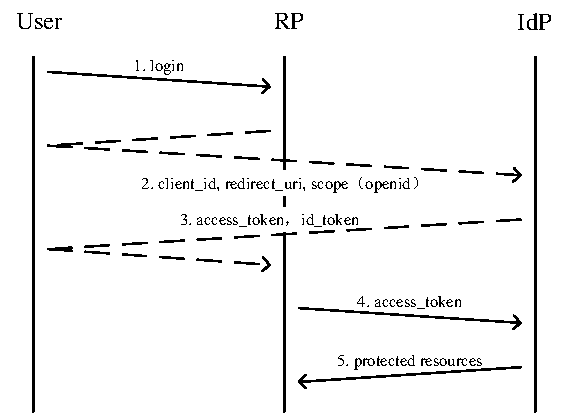
\includegraphics[width=\linewidth]{fig/implicit.pdf}\label{fig:OpenID}
  %\subfigure[Authorization Code Flow]{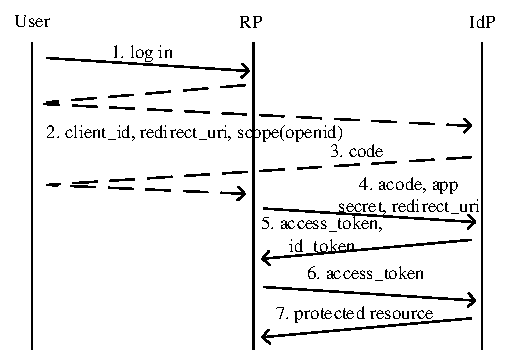
\includegraphics[width=\linewidth]{fig/openidconnect2.pdf}\label{fig:OpenID_code}}
  %\subfigure[Hybrid Flow]{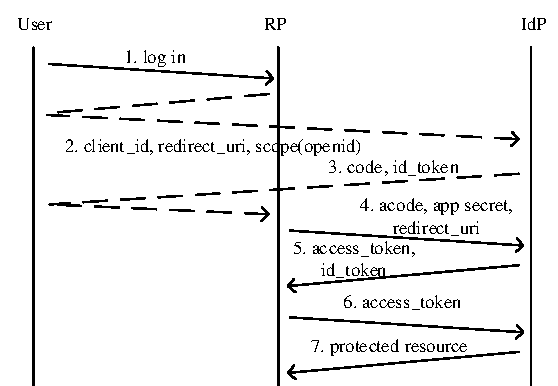
\includegraphics[width=\linewidth]{fig/openidconnect3.pdf}\label{fig:OpenID_hybrid}}
  \caption{The implicit protocol flow in OIDC.}
  \label{fig:OpenID}
\end{figure}

%Other Flows. Authorization code flow is similar to implicit flow. IdP firstly sends RP the authorization code instead of tokens. Then RP need use the code and a secret shared by RP and IdP to exchange for tokens with IdP. Hybrid flow is the combination of implicit flow and authorization code flow. RP is able to obtain code and token from IdP at the same time.
\end{comment}
\begin{comment}
\subsection{Security Consideration}
An RP must register a unique ID at IdP. To protect users' privacy, IdP should receive user's consent for specific RP before sending the PII to this RP. So IdP must get a valid ID from RP to represent RP's identity. And it has been discussed that the id token must be bound to the specific RP to avoid the reuse of token. It also requires that RP should provide the ID to IdP.

The redirect\_uri registered at IdP can avoid a malicious opponent to get a user's id token. IdP compares the redirect\_uri in the authentication request and uploaded during registration. Only when the redirect\_uri in the authentication has been uploaded during registration IdP is going to send the id token to requester. It guarantees that only the owner of the registered redirect\_uri is able to receive the id token issued for its registrant.


\subsection{Dynamic Registration}
Dynamic registration\cite{DynamicRegistration} is a function IdP provides RP to re-register its information at IdP. For dynamic registration, IdP issues each RP a registration token when the first registration of RP is finished. RP is able to register a new ID and redirect uri at IdP using the registration token.

To register a new RP at the IdP, firstly RP sends an HTTP POST message to the IdP with the parameters containing redirect uri, response type and other metadata parameters. This message is sent with the registration token. Upon successful registration, IdP generates a unique client id and returns it back with other registered metadata parameters.
\end{comment}


%流程

\begin{comment}
%\subsubsection{Analysis of OpenID Connect Flows}
%In OpenID Connect system, IdP is always able to get a user's login trace as it need to sign a id token with RP's id and user's id in it. Nist Special Publication 800-63C\cite{NIST} proposes that a user using the same IdP to authenticate to multiple RPs allows IdP to build a profile of user transactions.

%OpenID Connect 1.0 protocol is designed as extension protocol of OAuth 2.0 protocol. It can be seemed as an OAuth authentication version protocol. When OAuth protocol is firstly created there are other authentication protocols such as OpenID. So OAuth is specifically designed for user authorization. It allows third party to access user's personal protected resources from resource holder. Different from OpenID Connect 1.0, OAuth 2.0 usually offers two kinds of response type, code and token. In OAuth 2.0 protocol everyone carrying user's access token is able to achieve user's protected resources from resource holder. Access token is not bound with any RP so that it is not appropriate for authentication. It has been described in many works\cite{rfc6819}\cite{ChenPCTKT14}.
%Most of current IdPs\cite{Facebook} for web application use OAuth 2.0 authorization code flow. Because authorization code flow requires RP's secret for token exchanging. It actually achieves the binding of RP and access token. Although OAuth 2.0 implicit flow is not secure in authentication, many IdPs also use its modified version designed by each IdP for authentication.

%As OpenID Connect 1.0 is designed as an OAuth authentication version protocol, it can be used in both authentication and authorization. Id token is a security token that contains claims about authentication of a user for specific RP and it is represented as a JSON Web Token\cite{rfc7519}. In OpenID Connect 1.0 access token is mostly used for authorization. Id token is enough for user authentication. Code provides the benefit of not exposing id tokens to any malicious applications able to access user agent. Our protocol considers browser as the trust base so that authorization code flow is not necessary. We finally choose OpenID Connect 1.0 implicit flow with only response value of id\_token as the base of our enhanced protocol.

\subsection{Discussion of SSO System}
%OpenID Connect 1.0 protocol is designed as extension protocol of OAuth 2.0 protocol. When OAuth protocol is firstly created there are other authentication protocols such as OpenID. So OAuth is specifically designed for user authorization. It allows third party to access user's personal protected resources from resource holder. In OAuth 2.0 system everyone carrying user's access token is able to achieve user's protected resources from resource holder. Access token is not bound with any RP so that it is not appropriate for authentication.
%Most of current IdPs\cite{Facebook} for web application use OAuth 2.0 authorization code flow. Because authorization code flow requires RP's secret for token exchanging. It actually achieves the binding of RP and access token. Although OAuth 2.0 implicit flow is not secure in authentication, many IdPs also use its modified version designed by each IdP for authentication.

%为什么遵循openid connect,安全性得到了保证,已经被广泛使用
The reasons our privacy respecting single-sign-on protocol is designed based on OpenID Connect includes two main factors: 1) OpenID Connect 1.0 protocol and OAuth 2.0 protocol has been analysed in many previous works and they have been certified secure\cite{FettKS16}. So if the enhanced protocol can be insured as secure as OpenID Connect 1.0 protocol, it is deemed to be secure. 2) Current IdPs mostly use OAuth 2.0 and OpenID Connect 1.0 for user authentication\cite{Facebook}\cite{Google}. So it is convenient for developers to transfer their old system into the system with enhanced protocol if new protocol is similar with the previous one.

As OpenID Connect 1.0 is designed as an OAuth authentication version protocol, it can be used in both authentication and authorization. Id token is a security token that contains claims about authentication of a user for specific RP and it is represented as a JSON Web Token\cite{rfc7519}. In OpenID Connect 1.0 access token is mostly used for authorization. Id token is enough for user authentication. Code provides the benefit of not exposing id tokens to any malicious applications able to access user agent. Our protocol considers browser as the trust base so that authorization code flow is not necessary. We finally choose OpenID Connect 1.0 implicit flow with only response value of id\_token as the base of our enhanced protocol.

%单点登录系统中,IdP通过用户认证识别用户身份,通过client_id和redirect_uri识别RP身份。
%在不改变单点登录系统结构的情况下,由于IdP要向RP提供用户的身份信息,所以向IdP隐藏用户身份是不可行的
%向IdP隐藏RP身份要通过隐藏client_id和redirect_uri实现
%The ability of IdP. Discribe the solution of protecting users' privacy.
In OpenID Connect implicit flow, IdP gets a user's login trace in two ways. IdP gets RP's identity by client\_id and reditrct\_uri in redirect request (step 2) from RP. And IdP gets user's identity when authenticating the user (step 3). As IdP has to provide RP a user's authenticator bound with user's identity, it's not possible to keep user anonymous in IdP without modifying the structure of current SSO system. So it is only feasible to protect user's privacy by keeping RP anonymous in IdP. So it is needed to make client\_id and redirect\_uri unrelated with RP. But it introduces new challenges.

\subsubsection{Challenges}
%最直接的隐藏RP的方法是在登录过程中使用随机的client_id与redirect_uri
%简单的修改会带来两个方面的问题:流程问题与安全问题
%流程问题:IdP只识别注册过的client_id与redirect_uri;client_id与uid绑定,随机的client_id使每次的uid都不同
%安全问题:随机的client_id导致了不同RP之间的token可以混用;随机的redirect_uri导致IdP无法保证token只发送给对应的RP
%Security problems. The secure rules of sso system summarized from the previous research. And the simple solution will disobey which rules.
%Function problems. How the simple solution make the sso system failed.
%描述为何不能用户匿名
The simplest way to make RP anonymous in IdP is using random client\_id and redirect\_uri during each login. But the simple method will introduce some problems in two fields.

%关键句子表明问题的分类
Using random client\_id and redirect\_uri results in failure of authentication in current SSO system. IdP only accepts a request when the client\_id and redirect\_uri have been registered at IdP by an RP. So when using a random client\_id and redirect\_uri in a request, IdP will drop it as an invalid request. Additionally to protect user's privacy from RPs' collusion, it's required that IdP should provide different user\_ids for different client\_ids\cite{OpenIDConnect}. As a result, user\_id is bound to client\_id. While client\_id changing, user\_id changes. So a random client\_id for a RP means the user\_id is random too. If RP wants to provide a user personalize service user has to own a constant identity in RP. So randomness of client\_id means that RP can no more identify a user.

In the other field, anonymous RP causes secure problems. To avoid the misuse of id\_token among different RPs, RP judges the validation of id\_token through the client\_id in it. An client\_id represents a specific RP's identity, a id\_token with this client\_id is only valid in this specific RP. But when using a random client\_id, different RPs may share the same client\_id. When a user log in a malicious RP, this RP possibly logs in other RPs with the user's id\_token if they have the same client\_id. Additionally redirect\_uri is the address where RP waits for the id\_token. Before issuing a id\_token, IdP will check the validation of redirect\_uri to avoid attacker getting the id\_token. If the redirect\_uri is random, IdP can no more protect user from sending id\_token to an attacker.
\subsubsection{Solutions against the problems}
%通过协商生成client_id,任何一方无法控制client_id的生成
%用户代理控制token的发送,保证发送给对应的RP
%使用OpenID Connect 1.0的动态注册功能保证client_id与redirect_uri的有效性
%设计client_id与user id 的生成算法,使RP能够识别用户
With dynamic registration, a RP can register new random client\_id and redirect\_uri before sending a request to IdP for id\_token. And to avoid IdP finding out RP's identity through dynamic registration, the requirement of registration token is omitted. IdP will delete the expired registration to reduce storage stress.

To identify a user in different logins, RP must have the ability to transform the user\_id provided by IdP into a constant user identity for each user. Most of current SSO system generate user\_id as a random  character string. So a new user-id-generating algorithm has to be created for user authentication. As user\_id is required to be bound to random client\_id to protect from RPs' collusion, client\_id should be the primary input parameter to user-id-generating algorithm. To make user\_id able to be transformed into a constant user identity, it is a feasible way that generating client\_id through a client-id-generating algorithm. The user-id-generating algorithm and client-id-generating algorithm will be described detailedly in Section~\ref{sec:protocol}.

Misuse of id\_token only happens when different RPs use the same client\_id. Although IdP will keep the registered client\_id unique, an attacker is possible to be the executor of registration (RP or user) and tamper with the failed registration result. So victim will regard the repetitive client\_id as a validate one. To prevent misuse of id\_token, client-id-generating algorithm should require two random parameters respectively generated by RP and user. So even if an attacker possesses a user's id\_token (or negotiates a client\_id with RP), he is unable to negotiate the same client\_id with a RP (or get the id\_token with same client\_id from user).

As redirect\_uri is random, IdP is going to send id\_token to the invalidate address. User agent must intercept the id\_token redirection from IdP and send id\_token to RP. In PRISSO system IdP issues RP certification for each RP. A RP certification contains RP's identity and its address for token acceptance.  User gets the real acceptance address of RP from certification and makes sure that the id\_token is going to be sent to the RP. RP certification is also useful in defending phishing attack.
\end{comment}
